\documentclass[11pt,leqno,twoside]{article}
\usepackage{graphicx}
\usepackage{amsfonts}
\usepackage{enumerate}
\usepackage{amssymb}
\usepackage{hyperref}
\usepackage{amsmath}
\usepackage{bbm}
\usepackage{multirow}
\usepackage{enumerate}
\usepackage{natbib}
\setlength{\parskip}{1.2ex}        % space between paragraphs
\setlength{\parindent}{2em}        % amount of indention
\setlength{\textwidth}{7truein}      % default = 6.5"
\setlength{\oddsidemargin}{-12mm}   % default = 0"
\setlength{\evensidemargin}{-12mm}   % default = 0"
\setlength{\textheight}{225mm}     % default = 9"
\setlength{\topmargin}{-12mm}      % default = 0"
\usepackage[all]{xy}
\usepackage{tipa}
\input xy
\xyoption{all}
\usepackage{listings}
\newcommand{\indicator}[1]{\mathbbm{1}{\left[ {#1} \right] }}
\lstdefinelanguage{Scala}%
{morekeywords={abstract,case,catch,char,class,%
def,else,extends,final,%
if,import,%
match,module,new,null,object,override,package,private,protected,%
public,return,super,this,throw,trait,try,val,var,with%
},%
sensitive,%
morecomment=[l]//,%
morecomment=[s]{/*}{*/},%
morestring=[b]``,%
morestring=[b]',%
showstringspaces=false%
}[keywords,comments,strings]%

\lstset{language=Scala,%
mathescape=true,%
columns=[c]fixed,%
basewidth={0.5em, 0.40em},%
basicstyle=\tt,%
keywordstyle=\bfseries,%
}

\title{HW2: Regression}
\author{David Hall \\ \texttt{dlwh@cs.berkeley.edu}}
\begin{document}
\maketitle

\section{Introduction}

This report investigates the effect of optimization, objective
function, and regularization on a simple regression problem, namely,
the Amazon Books dataset described in \citet{Blitzer07Biographies}.

\section{Model and Optimization}

The model we use is a simple regularized regression model using either $\ell_2$ or $\ell_1$ loss and $\ell_2$ or $\ell_1$
regularization. That is, we seek to minimize, for $\{p,q\} \in \{1,2\}$ and tuning parameter $\lambda$:
\begin{equation*}
  \begin{split}
    \min_\theta \sum_i |y^{(i)} - \theta^T x^{(i)}|^p + \lambda ||\theta||_q^q
   \end{split}
 \end{equation*}
In our situation, each $y$ is the rating of a review (one of $\{1,2,4,5\})$ and $x$
is a bag-of-words of the review.
When $p=q=2$, we recover ridge regression, and when $p=2$ and $q=1$
we recover the ``lasso,'' which can obtain sparse solutions. While
exact solutions are possible for most of some of these conditions,
we instead focus on gradient-based optimizations.

Specifically, we consider two algorithms. First, we consider
the widely-used quasi-Newton method LBFGS~\citep{lbfgs}, and
the OWL-QN variant for $\ell_1$ regularization~\citep{Andrew07scalabletraining}.
Second, we consider the Adaptive Gradient (AdaGrad) variant of Stochastic Gradient Descent,
using forward $\ell_2$ and $\ell_1$ regularization.~\citep{duchi10adaptive}. This latter algorithm
is much like gradient descent, except that step sizes are determined on a per-component basis, where
the step size at time $t$ for component $i$ is defined to be:
\begin{equation}
  \begin{split}
    \alpha_{ti} &= \frac1{\delta + \sum_{t'=1}^t g_{t'i}^2}
   \end{split}
 \end{equation}
 where $g_{ti}$ is the gradient of component $i$ at time $t$. Forward regularization complicates the
 update slightly. We direct the reader to \citet{duchi10adaptive} for a thorough description, including
 the actual updates for both $\ell_1$ and $\ell_2$ regularization.

\section{Experimental Setup}

We use all of the reviews in the Books dataset, using the top 40000
most common words after removing stop words. No attempt was made
to remove duplicates, and no additional features were added beyond
the raw word counts. We perform a 10-fold cross-validation, as requested.

All implementations of the algorithms are just the ScalaNLP
implementations of these algorithms.\footnote{\url{http://scalanlp.org/}.
Hey, I wrote it!}.  The only new code was for reading in the dataset,
removing stop words, and the objective function. We parallelized
the objective using the Scala-built-in fork/join framework described
in \citet{prokopec2011Generic}. For the AdaGrad updates, we used a
batch size of 4096, which was sufficient to saturate two cores of
a modern Intel i7 processor. (LBFGS was able to use all four cores.)
We use a regularization constant $\lambda$ of 1E-4. We did not
attempt to tune this parameter, except that $\lambda = 1$ clearly
underperformed.

For metrics, we focus on Root Mean Square Error (RMSE) as well as
classification F1, where the classification task is defined as
correctly determining a review as positive (rating of 4 or 5) or
negative (rating of 1 or 2).

\section{Experiments}

We conduct three experiments. First, we plot test RMSE as a function
of the number of passes through the data. Second, we consider
classification performance for both $\ell_1$ and $\ell_2$ losses
and regularization. Finally, we are interested the sparsity associated
with the different executions.

\subsection{Convergence rates}
\begin{figure}
  \centering
  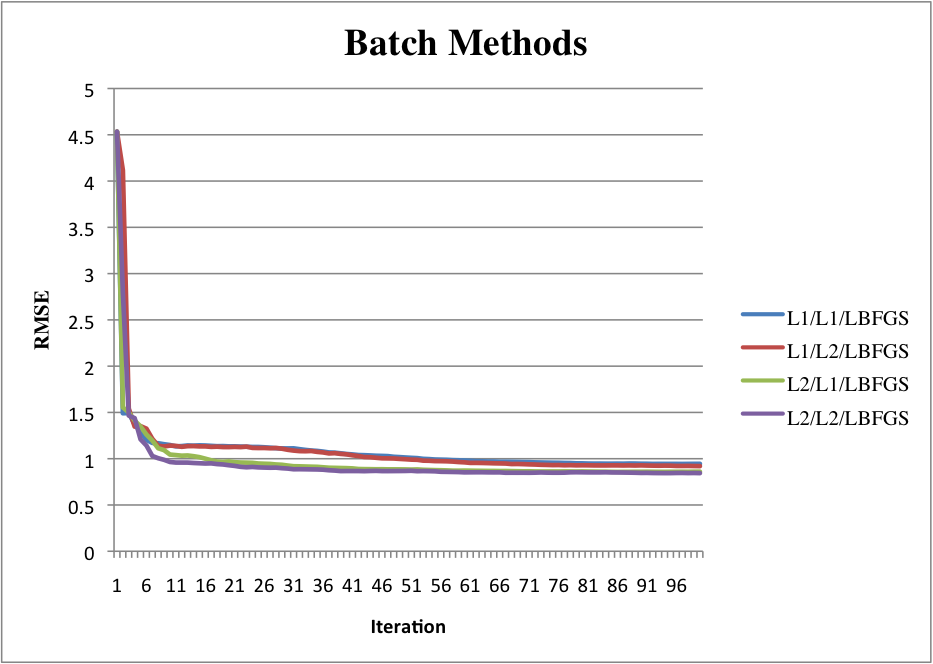
\includegraphics[scale=0.49]{lbfgs-rmse.png}
  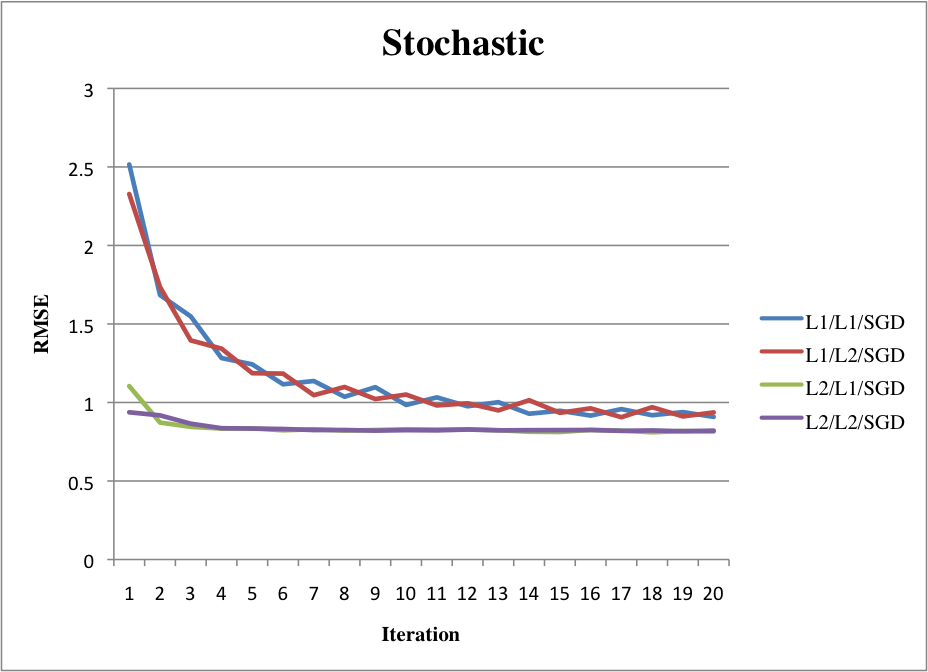
\includegraphics[scale=0.49]{stochastic-rmse.png}
  \caption{Batch and Stochastic optimization RMSE as a function of iteration}
  \label{fig:rmse-stochastic}
\end{figure}

In Figure \ref{fig:rmse-stochastic} we plotted the average test-set
RMSE across validation runs, as a function of pass through the data
for the batch and stochastic methods, respectively. Unsurprisingly,
the $\ell_2$ methods are better at minimizing RMSE, since they are
optimizing the actual evaluation criterion.

As is generally observed in the literature, SGD is much faster than LBFGS,
achieving optimal performance in just 5 iterations for the $\ell_2$
losses. $\ell_1$ loss takes a little longer, which is not surprising
since it is not smooth. Indeed, the stochastic $\ell_1$ methods
clearly show a significant amount of ``bouncing around,'' while the
$\ell_2$ methods converge much more quickly.

It is actually surprising to see $\ell_1$ loss behave as well as
it does with LBFGS and OWL-QN, which is typically quite sensitive to discontinuities
and more generally errors in the gradient in our prior experience.
We did observe that LBFGS had to choose smaller step sizes more frequently
for the $\ell_1$ loss updates.

In terms of final performance, $\ell_2$/$\ell_1$ performed the best
with an RMSE of 0.815, while $\ell_2/\ell_2$ was not far behind at
0.821. The $\ell_1$ objectives were around 0.91-0.92, which again
is unsurprising since they were not optimizing that metric.

\subsection{Classification Performance}
\begin{table}
\centering
  \begin{tabular}{|c|c|c|c|}
    \hline
    Obj. & Reg. & Micro & Macro \\
    \hline
    $\ell_1$ & $\ell_1$ & 0.917 & 0.742 \\
    $\ell_1$ & $\ell_2$ & 0.912 & 0.752 \\
    $\ell_2$ & $\ell_1$ & 0.942 & 0.841 \\
    $\ell_2$ & $\ell_2$ & 0.937 & 0.822 \\
    \hline
  \end{tabular}
  \caption{Micro- and Macro-averaged F1 scores for different combinations of regularization and objective.}
  \label{tbl:classification}
\end{table}


We then considered the classification performance for each of the
objectives and regularization settings. We report micro- and macro-averaged
F1, to account for the fact that most reviews are positive. All scores
are averaged over the 10 runs. Table \ref{tbl:classification} contains the results.

Interestingly, the $\ell_2$ objective also outperforms the $\ell_1$
on classification accuracy, as well as on RMSE. Perhaps this could
be fixed by improving the regularization constant, but we do not
pursue that here.

\subsection{Sparsity}
$\ell_1$ regularization is generally known for producing sparse solutions. We investigated
the claim empirically by comparing the number of zero entries in the weight vector for both $\ell_2$
and $\ell_1$ regularization using SGD. $\ell_2$, as predicted, did not produce a sparse solution, 
with more than 99\% of the parameters having a non-zero weight. However, using $\ell_1$ regularization,
only 46\% of the parameters have non-zero weight. 

\subsection{High Weight Terms}
\begin{table}
  \centering
  \begin{tabular}{|c|c|}
    \hline
    Term & Weight \\
    \hline
boring  &  -0.3583\\
waste  &  -0.3565\\
excellent  &  0.321\\
disappointed  &  -0.269\\
money  &  -0.263\\
bad  &  -0.261\\
disappointing  &  -0.2597\\
wonderful  &  0.2413\\
best  &  0.2362\\
worst  &  -0.2285\\
$<$/title$>$   &  0.225\\
$<$date$>$   &  0.225\\
$<$/date$>$   &  0.225\\
$<$title$>$   &  0.225\\
$<$reviewer$>$   &  0.225\\
$<$/reviewer$>$   &  0.225\\
$<$review$>$   &  0.225\\
$<$/reviewer\_location$>$   &  0.225\\
$<$review\_text$>$   &  0.225\\
$<$/review\_text$>$   &  0.225\\
    \hline
  \end{tabular}
    \caption{Terms with the highest weight in terms of absolute value from our model.}
    \label{tbl:weights}
\end{table}

Just as an interesting visualization exercise, we print the top
twenty terms with the highest absolute weight from the $\ell_2/\ell_1$
configuration, in Table \ref{tbl:weights}. Many of the words are
obviously correlated with high or low reviews. ('money' is fairly
negative, which is pretty funny, really!) The xml tags are basically
bias features: they appear in every document, and the dataset is
fairly biased to positive reviews.

\section{Conclusion}

We examined the effect of various modifications to optimization, regularization, and objective
on a simple regression task. We demonstrated known previously known results: that stochastic
methods are typically faster than batch methods, and that $\ell_1$ regularization can lead to sparsity. Interestingly,
we also found that $\ell_1$ loss is not as effective for the classification loss as $\ell_2$.



\bibliographystyle{plainnat}
\bibliography{refs}
\end{document}
